\section{REST API}
Vores API består af 3 dele;
\begin{itemize}
    \item Controllers der opsætter REST endpoints og konvertere data fra URLencoded / JSON til C\# objekter.
    \item Services der connecter til de forskellige databaser, og om skriver dataen til queries.
    \item Databaserne som er opsat som cluster og single containers hvis cluster ikke er muligt.
\end{itemize}
På figur \ref{fig::api} har vi REST API’et med alle controllerens endpoints helt til venstre, efterfulgt af alle services’ som håndtere dataen og sender det til den rigtige database. Alle endpoints, udover logs, går igennem “Create Log” servicen som skriver til HBASE. Udover dette har vi også 2 cache services’ som flusher og checker om en cache findes inden den går til databasen for at finde dataen.

\begin{figure}[H]
    \centering
    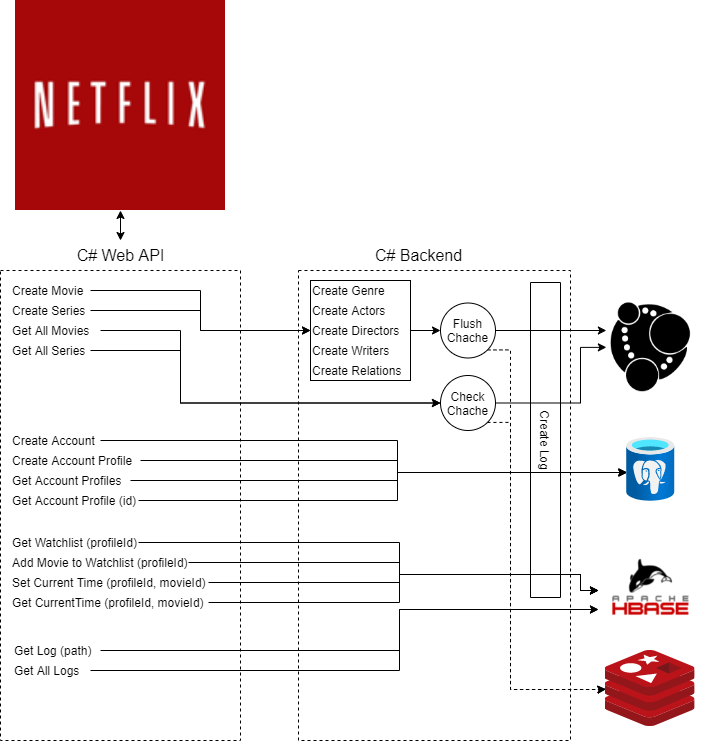
\includegraphics[scale=0.60]{api.png}
    \caption{REST API Model}
    \label{fig::api}
\end{figure}